%%%% Relay pitch deck — Snapdragon AI Lab Build & Present Challenge.
%%%% Theme by LianTze Lim (April 2017), reused as-is per the author's own
%%%% preferred Beamer style from a prior project.

\documentclass[12pt]{beamer}

\usepackage[english]{babel}
\usepackage[utf8]{inputenc}
\usepackage[T1]{fontenc}
\usepackage{lmodern}
\usepackage{tikz}
\usetikzlibrary{arrows.meta,positioning,shapes.multipart}
\usepackage{booktabs}
\usepackage{tabularx}
\newcolumntype{Y}{>{\raggedright\arraybackslash}X}

\makeatletter

\setbeamersize{text margin left=1em,text margin right=1em}

\setbeamerfont{title}{series=\bfseries,size=\LARGE}
\setbeamerfont{subtitle}{series=\bfseries,size=\Large}
\setbeamerfont{frametitle}{series=\bfseries,size=\small}
\setbeamerfont{block title}{series=\bfseries,size=\normalsize}
\setbeamerfont{footline}{size=\normalsize}

\usebeamercolor{structure}
\setbeamercolor{normal text}{fg=structure.fg}

\addtobeamertemplate{frametitle}{}{\vspace*{-1ex}\rule{\textwidth}{1pt}}

\setbeamertemplate{itemize items}[circle]

\setbeamertemplate{navigation symbols}{}

\setbeamertemplate{footline}{%
   \centering
   \begin{minipage}{\dimexpr\paperwidth-\beamer@leftmargin-\beamer@rightmargin\relax}
   \centering
   \rule{\linewidth}{1pt}\vskip2pt
   \usebeamerfont{footline}%
   \usebeamercolor{footline}%
   \hfill\insertpagenumber/\inserttotalframenumber
   \hfill%
   \llap{\insertframenavigationsymbol\insertbackfindforwardnavigationsymbol}\par
   \end{minipage}\vskip2pt
}

\makeatother

\title{Relay}
\subtitle{An On-Device, Voice-Controlled, Screen-Reading Accessibility Agent}
\author{Kartik Pandey}
\institute{IIIT Naya Raipur}
\date{Snapdragon AI Lab Build \& Present Challenge, September 2026}

\begin{document}

\begin{frame}
  \titlepage
\end{frame}

\begin{frame}{Outline}
  \tableofcontents
\end{frame}

\section{Introduction}

\begin{frame}{The Problem}

\begin{itemize}
  \item People with \textbf{limited hand mobility or low vision} can't
    reliably operate a Windows PC through a mouse and a screen alone.
  \item Existing screen readers \emph{describe} a screen but don't act on
    it; existing automation agents act, but weren't built around this
    population's safety needs.
  \item \textbf{Idea:} a voice-first agent that both understands the
    screen and acts on it --- with a person narrating every step, and a
    spoken confirmation gate on anything consequential.
\end{itemize}

\vskip 0.5cm

\begin{block}{Design goals}
On-device only, no cloud round-trip for speech or screen understanding
$\cdot$ never act on anything sensitive without a spoken ``yes''
$\cdot$ scoped assistive technology, not a general autonomous agent
\end{block}

\end{frame}

\begin{frame}{Why Not Just Use a General Computer-Use Agent?}

\begin{itemize}
  \item General autonomous agents can already read a screen and click or
    type on it.
  \item But the cost of being wrong is asymmetric:
  \begin{itemize}
    \item Agent mis-clicks a harmless button $\rightarrow$ annoying, but
      recoverable.
    \item Agent confidently taps ``Send'' / ``Delete'' / ``Pay'' on a
      misread screen $\rightarrow$ real, sometimes irreversible harm.
  \end{itemize}
  \item $\Rightarrow$ the whole design is biased toward \textbf{safety
    over autonomy}: nothing consequential executes without a spoken
    confirmation, ever.
\end{itemize}

\end{frame}

\section{Pipeline Overview}

\begin{frame}{End-to-End Pipeline}

\begin{center}
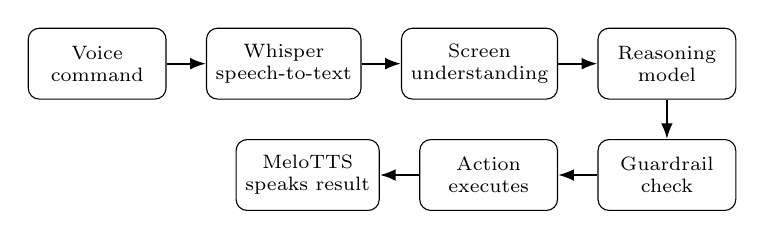
\begin{tikzpicture}[
  node distance=0.5cm and 0.5cm,
  every node/.style={draw, rounded corners, align=center, font=\scriptsize,
                      minimum height=0.9cm, minimum width=1.75cm},
  arr/.style={-{Latex[length=2mm]}, thick}
]
\node (voice) {Voice\\command};
\node (whisper) [right=of voice] {Whisper\\speech-to-text};
\node (screen) [right=of whisper] {Screen\\understanding};
\node (reason) [right=of screen] {Reasoning\\model};
\node (guard) [below=of reason] {Guardrail\\check};
\node (act) [left=of guard] {Action\\executes};
\node (tts) [left=of act] {MeloTTS\\speaks result};

\draw[arr] (voice) -- (whisper);
\draw[arr] (whisper) -- (screen);
\draw[arr] (screen) -- (reason);
\draw[arr] (reason) -- (guard);
\draw[arr] (guard) -- (act);
\draw[arr] (act) -- (tts);
\end{tikzpicture}
\end{center}

\vskip 0.3cm
\begin{itemize}
  \item Screen understanding checks the UI Automation accessibility tree
    first; only falls back to a vision-language model when that tree
    doesn't have enough named, enabled controls to work with.
  \item The guardrail check never changes: two-tier ALLOW / CONFIRM /
    BLOCK against pattern-matched control names, evaluated
    \emph{before} any action executes.
\end{itemize}

\end{frame}

\section{Screen Understanding}

\begin{frame}{The Fast Path --- UI Automation Tree}

\begin{itemize}
  \item Reads the live accessibility tree first: named, enabled controls,
    no model call needed.
  \item Verified against real, live windows on this machine:
  \begin{itemize}
    \item \textbf{Media Player} --- 211 elements, 113 named + enabled,
      real actionable content (Search, Open file(s), Recent media).
    \item \textbf{Notepad} --- a simple-app proxy, 24 elements, a real
      scroll action executed successfully.
  \end{itemize}
  \item Falls back to a vision-language model only when the tree
    genuinely doesn't have enough to work with --- not the common case,
    the exception.
\end{itemize}

\end{frame}

\begin{frame}{The Chromium Gap --- Found, Verified, and Fixed}

\begin{itemize}
  \item \textbf{Edge and Outlook} are both Chromium/WebView2-based:
    walking their UI Automation tree 12--14 levels deep surfaces window
    chrome only --- \textbf{zero} real page content, confirmed, not
    assumed.
  \item \textbf{Fixed for Edge} via the Chrome DevTools Protocol: real
    page content read from a live Wikipedia page, a real value typed
    into the real search box, and the write independently confirmed by
    re-reading the live DOM afterward.
  \item Outlook's equivalent gap remains open --- it's a desktop app, not
    a browser tab the DevTools Protocol can attach to.
\end{itemize}

\vskip 0.2cm
{\small
\begin{block}{Every claim here is labeled by how it was verified}
Run on real hardware/software, confirmed from real source code, or
explicitly marked as not yet possible without Snapdragon-class hardware.
\end{block}
}

\end{frame}

\section{The Guardrail Engine}

\begin{frame}{Two-Tier Decision}

\begin{itemize}
  \item Every decision is checked against the target control's name
    \emph{before} it executes:
\end{itemize}

{\small
\[
  \text{decision} =
  \begin{cases}
    \textsc{Block}   & \text{name matches a block pattern (irreversible)} \\
    \textsc{Confirm} & \text{name matches a confirm pattern (consequential)} \\
    \textsc{Allow}   & \text{otherwise}
  \end{cases}
\]
}

\begin{itemize}
  \item \textsc{Confirm}: send/submit/post/publish, pay/buy/transfer,
    delete/remove/erase, account or security changes --- requires a
    spoken ``yes'' before proceeding.
  \item \textsc{Block}: factory reset, reformat, disabling the firewall
    or antivirus --- never executes, no override.
  \item Every decision is written to a persisted, append-only audit log.
\end{itemize}

\end{frame}

\begin{frame}{Adversarial Testing}

\begin{itemize}
  \item 18 adversarial test cases built from plausible real controls
    across all three target apps.
  \item Found a genuine gap: the pattern
    \texttt{\textbackslash bdelete\textbackslash b}'s word boundary
    didn't match inside ``deleted'' --- so a real control like ``Empty
    deleted items folder'' silently fell through to \textsc{Allow}.
  \item Fixed by widening \texttt{delete}/\texttt{remove}/\texttt{erase}
    to also catch \texttt{-ed}/\texttt{-ing}/\texttt{-ion} forms --- a
    widening, never a narrowing, by design: these patterns should get
    harder to change, not easier.
\end{itemize}

\end{frame}

\begin{frame}{The Full Decision Flow}

\begin{center}
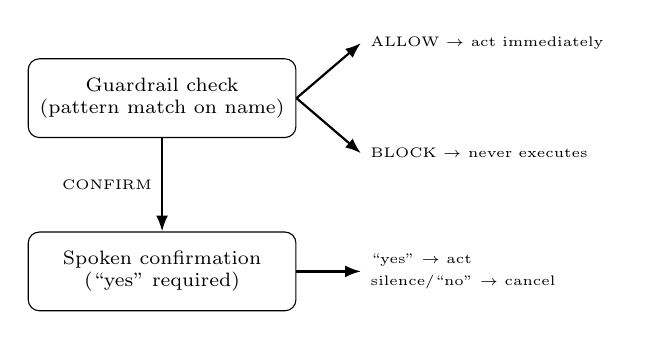
\begin{tikzpicture}[
  box/.style={draw, rounded corners, align=center, font=\scriptsize,
              minimum height=1cm, minimum width=3.4cm},
  outlbl/.style={align=left, font=\tiny, text width=3.3cm},
  arr/.style={-{Latex[length=2mm]}, thick}
]
% Explicit coordinates — a "below/right of" layout with the positioning
% library collided two of the output labels here (found only by actually
% rendering the slide: "BLOCK" and "never executes" overlapped
% illegibly), so this diagram is laid out on fixed coordinates instead,
% giving each label a guaranteed-clear row.
\node[box] (guard) at (0,0) {Guardrail check\\(pattern match on name)};
\node[box] (confirm) at (0,-2.2) {Spoken confirmation\\(``yes'' required)};

\node[outlbl] (allow) at (4.3,0.7)  {ALLOW $\rightarrow$ act immediately};
\node[outlbl] (block) at (4.3,-0.7) {BLOCK $\rightarrow$ never executes};
\node[outlbl] (yes)   at (4.3,-2.2) {``yes'' $\rightarrow$ act\\[2pt]silence/``no'' $\rightarrow$ cancel};

\draw[arr] (guard) -- node[left,font=\tiny]{CONFIRM} (confirm);
\draw[arr] (guard.east) -- (allow.west);
\draw[arr] (guard.east) -- (block.west);
\draw[arr] (confirm.east) -- (yes.west);
\end{tikzpicture}
\end{center}

\vskip 0.2cm
\begin{itemize}
  \item Most decisions resolve immediately (ALLOW or BLOCK).
  \item Only genuinely consequential actions pay the extra cost of a
    spoken confirmation round-trip.
\end{itemize}

\end{frame}

\section{Implementation}

\begin{frame}{What's Actually Real}

\begin{itemize}
  \item \textbf{Whisper speech-to-text} --- real transcription of a
    known test clip, reproduced three independent ways.
  \item \textbf{MeloTTS-EN} --- real synthesis, real audio, played back
    through real speakers (five independent real blockers found and
    fixed to get there).
  \item \textbf{The full \texttt{agent.py} orchestration loop} --- a
    real mic recording $\rightarrow$ real transcription $\rightarrow$
    real UI Automation tree read $\rightarrow$ real guardrail gate
    $\rightarrow$ real action $\rightarrow$ real speech, proven end to
    end against a live window. Only the NPU-dependent reasoning step is
    mocked.
  \item \textbf{\texttt{cdp\_perception.py}} --- the Chrome DevTools
    Protocol fix for Edge, wired into \texttt{agent.py}'s real
    orchestration and demonstrated live.
\end{itemize}

\end{frame}

\section{Results}

\begin{frame}{Competitive Differentiation}

\begin{table}
\centering
\scriptsize
\begin{tabularx}{\textwidth}{@{} >{\raggedright\arraybackslash}p{1.7cm} Y >{\raggedright\arraybackslash}p{2.6cm} @{}}
\toprule
\textbf{Project} & \textbf{Safety mechanism} & \textbf{Enforcement} \\
\midrule
Deft         & None found anywhere in either backing repo & N/A \\
Orbit        & None --- but never takes actions at all & N/A \\
ScreenSaathi & Keyword list downgrades risky plans & Code-level \\
Sally        & A prompt asking the model nicely & Model-enforced only \\
\textbf{Relay} & \textbf{ALLOW / CONFIRM / BLOCK + spoken yes + audit log} & \textbf{Code-level, pre-execution} \\
\bottomrule
\end{tabularx}
\caption{Verified against each project's real, public source code --- not a secondhand summary.}
\end{table}

\begin{itemize}
  \item Of five comparable projects, Relay is the only one with a
    deterministic, code-level safety gate that doesn't depend on a
    language model correctly following an instruction.
\end{itemize}

\end{frame}

\begin{frame}{Real Snapdragon Hardware --- Qualcomm AI Hub}

\begin{table}
\centering
\begin{tabular}{lc}
\toprule
\textbf{Metric} & \textbf{Value} \\
\midrule
Whisper-base encoder & $\sim$49.1~ms \\
Whisper-base decoder & $\sim$3.7~ms \\
\bottomrule
\end{tabular}
\caption{Compiled and profiled on a real Snapdragon X Elite CRD via Qualcomm AI Hub's hosted device farm.}
\end{table}

\begin{itemize}
  \item A real compile + profile job on actual target silicon --- not a
    simulation, and an order of magnitude faster than this laptop's CPU.
  \item Precisely scoped: this is AI Hub's compile/profile path, not yet
    a full GenieX runtime measurement, which needs physical device
    access.
\end{itemize}

\end{frame}

\section{Limitations \& Future Work}

\begin{frame}{Honest Roadmap}

\begin{itemize}
  \item \textbf{Open:} Outlook's Chromium accessibility gap --- the same
    limitation as Edge, but it's a desktop app the DevTools Protocol
    can't attach to. Unsolved, documented as such.
  \item \textbf{Open:} full GenieX-runtime, on-device latency for the
    reasoning model --- needs physical Snapdragon hardware, not yet
    measured.
  \item \textbf{Done:} 18 adversarial guardrail tests, a fixed task-list
    harness (100\% pass rate, 5/5), and short-term reasoning memory
    (last 3 turns).
  \item This submission was built without physical Snapdragon hardware
    --- every claim in this deck is labeled by exactly how it was
    verified.
\end{itemize}

\vskip 0.5cm
\centering
\small \texttt{github.com/kartik1pandey/relay-accessibility-agent}

\end{frame}

\end{document}
